% !TEX root =  ../main.tex 

\section{Simulation study}
\label{sec: simulation_study}
The application of personalized schedules for patients in PRIAS demonstrated that personalized schedules adapt according to the history of each patient. However, since the patients in PRIAS have already had their biopsies as per the PRIAS schedule, we were not able to evaluate the efficacy of personalized schedules against the PRIAS schedule. To this end, we have performed a simulation study to compare 3 broad categories of schedules: Personalized schedules, PRIAS schedule and a schedule of annual biopsy.

\subsection{Simulation setup}
\label{subsec : simulation_setup}
In the simulation study we used a total of 100 data sets with 1000 patients each. For each of the patients in the 100 data sets, we generated the longitudinal profiles using the posterior estimates of the parameters $p(\boldsymbol{\theta} \mid \mathcal{D}^{PRIAS})$ from the joint model fitted to the PRIAS data set (Section \ref{subsec : jm_fit_prias}). The visit times for PSA measurements were the same as PRIAS schedule. i.e. Every 3 months for first 2 years and every 6 months thereafter. Similarly, while generating Gleason reclassification times for the patients, the parameters of the linear predictor in the hazard function (Equation \ref{eq : hazard_prias}) were obtained from the joint model fitted to PRIAS data set. However unlike the flexibly modeled baseline hazard in PRIAS joint model, the baseline hazard in the simulation study was modeled using a Weibull distribution. We used 10 sets of parameters $\Omega_g = \{\lambda_g, k_g\}; g = 1,... 10$ for the Weibull baseline hazard, one each for a group $g$ of 10 data sets. This was done, firstly to ensure that different data sets $\mathcal{D}^g_k; k = 1, ...10$ within a group are sampled from the same population $\mathcal{P}_g$ of patients. This way we could isolate the variation in the performance of a scheduling method. Secondly, different parameter values for the baseline hazard across the groups ensured that we tested different patient populations; those who have early progression times, as well as those who have late progression times. This is important because how late or early patients are observed to have GR, partly depends on the induction criteria of the AS program. (\textcolor{red}{\textbf{Give the values of $\Omega$ for different populations and the corresponding histograms of GR times.}})\\

In a real life scenario the parameters $\boldsymbol{\theta}$ of a joint model for hazard of GR and PSA measurements will not be known in advance, and hence we do not use posterior estimates $p(\boldsymbol{\theta} \mid \mathcal{D}^{PRIAS})$ from the joint model fitted to the PRIAS data set to create personalized schedule for the simulated patients. Instead we divide each of the 100 simulated data sets into training (750 patients) and test (250 patients) parts. For ease of notation we reuse $\mathcal{D}^g_k$ as the notation for the $k^{th}$ training data set from the $g^{th}$ group. Further we simulate random and non-informative censoring times for the patients in training data set. Thus $\mathcal{D}^g_k = \{T_i, \delta_i, \boldsymbol{y}_i; i = 1,...750\}$. $T_i = \min(T_i, C_i)$ denotes the observed GR time for the $i^{th}$ patient in training data set. $\delta_i = I(T_i < C_i)$ is the event indicator, where $I(\cdot)$ is an indicator function that takes the value 1 when $T_i < C_i$ and 0 otherwise. We then fit a joint model to the training data set to obtain posterior estimates of parameters $p(\boldsymbol{\theta} \mid \mathcal{D}^g_k)$, which are required for the predictive distribution $g(T^*_j)$ of the $j^{th}$ patient from the test data set. To create the personalized schedules, we use the algorithm described in Section \ref{subsubsec : pers_sched_algorithm}.

\subsection{Evaluating efficacy of scheduling methods}
For a given population of patients $\mathcal{P}_g$, the first criteria in evaluation of efficacy of a schedule $S$ for biopsies is the number of repeat biopsies $N^S_g$ it takes before GR is detected for a patient from the population. The less $N^S_g$ the better it is for patients. In case of annual schedule, $N^S_g$ depend only on the true GR time $T^*_g$ of a patient. On the other hand, for PRIAS and personalized schedules $N^S_g$ depend on PSA measurements $\boldsymbol{y}_g$ as well as on true GR time. In either case, the marginal distribution of the number of biopsies $p(N^S_g)$ for the entire population is unknown. We estimate the mean and quantiles of this distribution from the observed number of biopsies $N^S_{g_{kj}}; j=1,...250$ for each of the 250 test patients in the $k^{th}$ data set of the $g^{th}$group (\textcolor{red}{\textbf{Should we instead take mean of means using the 10 data sets?}}). The second criteria in evaluation of efficacy of a schedule is the offset $O^S_g = T^S_g - T^*_g$, where $T^S_g > T^*_g$ is the time at which GR is detected by the scheduling mechanism $S$. Once again the marginal distribution $p(O^S_g)$ is not known. We estimate the mean and quantiles of this distribution from the observed offset $O^S_{g_{kj}}; j=1,...250$ for each of the 250 test patients in the $k^{th}$ data set of the $g^{th}$group.\\

Certain scheduling mechanisms may have a smaller mean offset $E[O^S_g]$, but they may schedule a lot of biopsies. One such schedule is the annual repeat biopsy schedule. No matter what the GR time for a patient is, the offset will never be more than 1 year. The vice versa of this scenario is also possible. Given the medical aspects of biopsies, it is not possible to prefer one criteria over another. For e.g. A doctor may choose a schedule with the least mean number of biopsies possible as long as the mean offset is below a certain threshold; such as 3 years in PRIAS. But certain schedules have a small mean offset $E[O^S_g]$, while simultaneously having a high variance $Var[O^S_g]$. i.e. the scheduling mechanism is not suitable for everyone in the population. In such a case the doctor may put a threshold on offset not being larger than a certain number of months for $p$\% of the patients. The choice of $p$ can be done on the basis of patient's consent or an AS program's policy.

\subsection{Results}
Since the Gleason reclassification times varied widely across the simulation data sets, we discuss the results separately for the different scenarios. In total we have 6 scenarios corresponding to the 6 groups of 10 data sets. For brevity, we only chose 3 most dissimilar scenarios and further we present one set of results for each of the 3 scenarios. The complete set of results can be found at \url{https://goo.gl/u6dg8G}. At this moment, we will not compare our results against the PRIAS schedule, since the PRIAS schedule we used is fixed for all patients, whereas in reality it can be dynamic if the PSA doubling time is less than 10 years.

\subsubsection{Scenario 1}
In the first scenario the Gleason reclassification times for the patients are mostly between 7 and 11 years. The Gleason reclassification times of test patients from one of the data sets is shown in Figure \ref{fig : sc_10_sh_7pt5_progression_hist}. Figure \ref{fig : sc_10_sh_7pt5_offset_boxplot} shows that, for this data set the approaches with the least number of biopsies, 2 in number, are conditional expected failure time, and dynamic risk with a threshold $\kappa$ chosen such that accuracy (section \ref{subsubsec : dynamic_risk_definitions}) is maximized. The mean and median offset for the two approaches is around 9 months. However for a few outlying patients the offset is more than 24 months. If we compare this to the schedule of performing biopsy every year the mean offset is around 6 months and mean number of biopsies is 8. 

\begin{figure}[H]
\centering
\captionsetup{justification=centering}
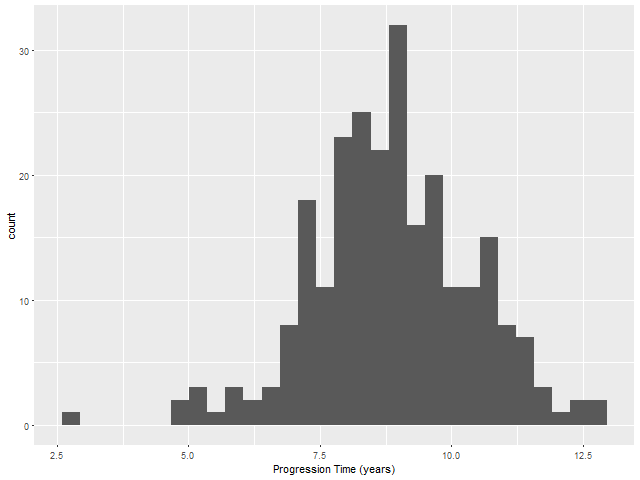
\includegraphics[width=0.8\textwidth]{sim_study_res_sc_10_sh_7pt5/progression_hist.png}
\caption{\label{fig : sc_10_sh_7pt5_progression_hist} Gleason reclassification times for patients from the test data set of scenario 1.}
\end{figure}

\begin{figure}[H]
\centering
\captionsetup{justification=centering}
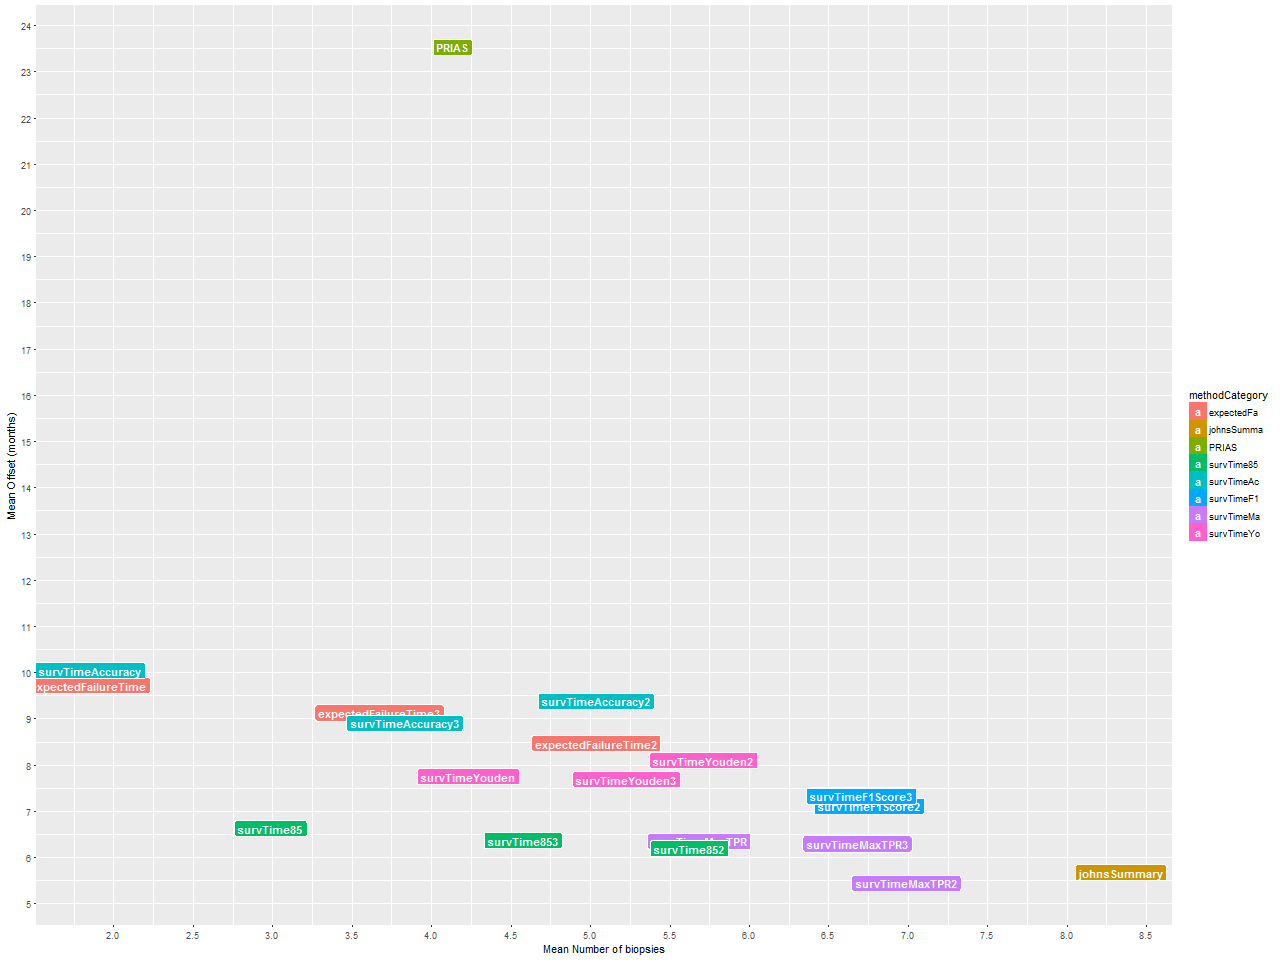
\includegraphics[width=\textwidth]{sim_study_res_sc_10_sh_7pt5/mean_offsetvsnb.png}
\caption{\label{fig : sc_10_sh_7pt5_mean_offsetvsnb} Mean number of biopsies against the mean offset (in years) for each of the approaches in scenario 1.}
\end{figure}

\begin{figure}[H]
\centering
\captionsetup{justification=centering}
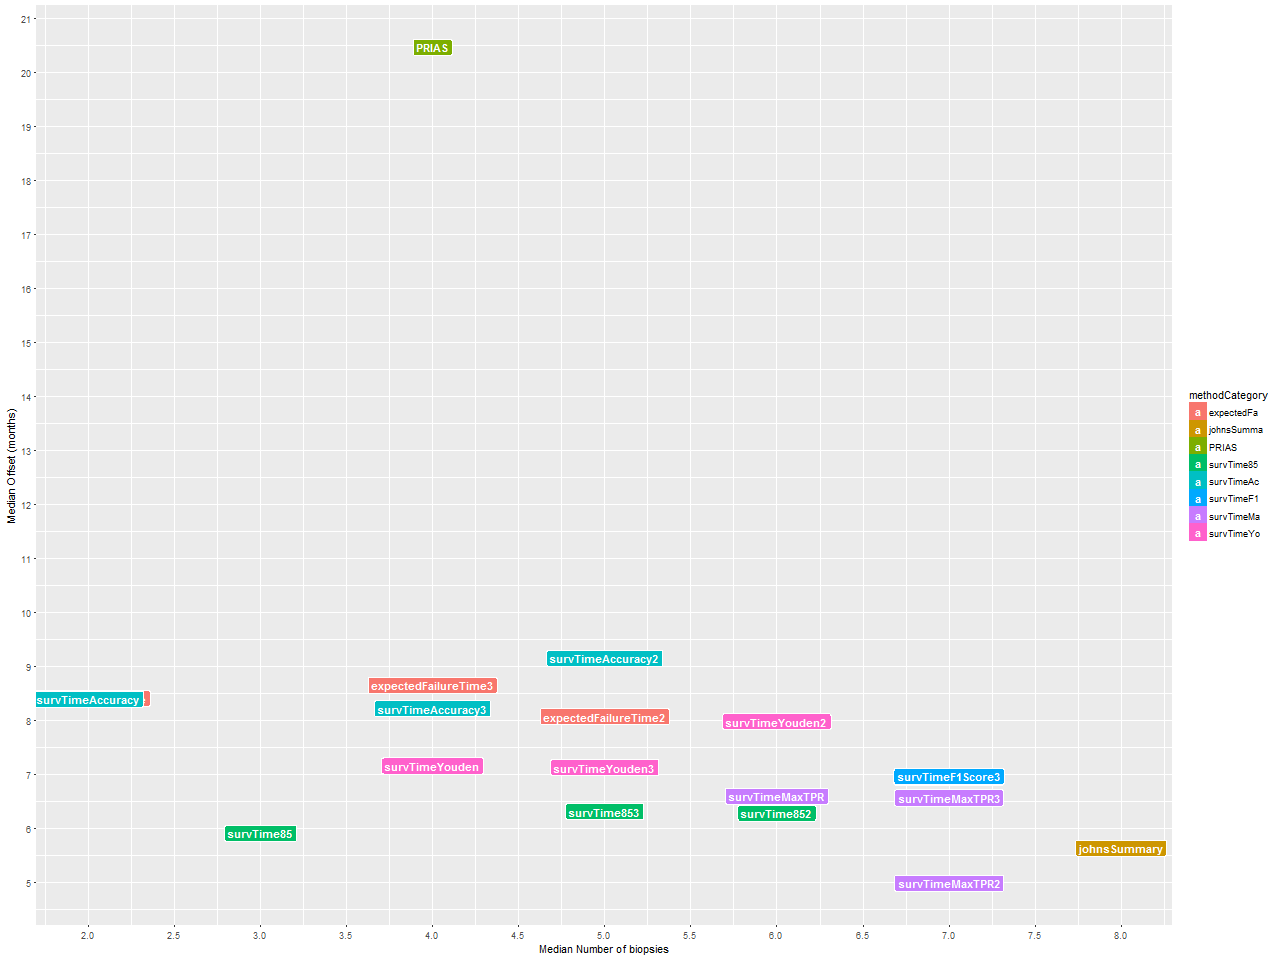
\includegraphics[width=\textwidth]{sim_study_res_sc_10_sh_7pt5/median_offsetvsnb.png}
\caption{\label{fig : sc_10_sh_7pt5_median_offsetvsnb}Median number of biopsies against the median offset (in years) for each of the approaches in scenario 1.}
\end{figure}

\begin{figure}[H]
\centering
\captionsetup{justification=centering}
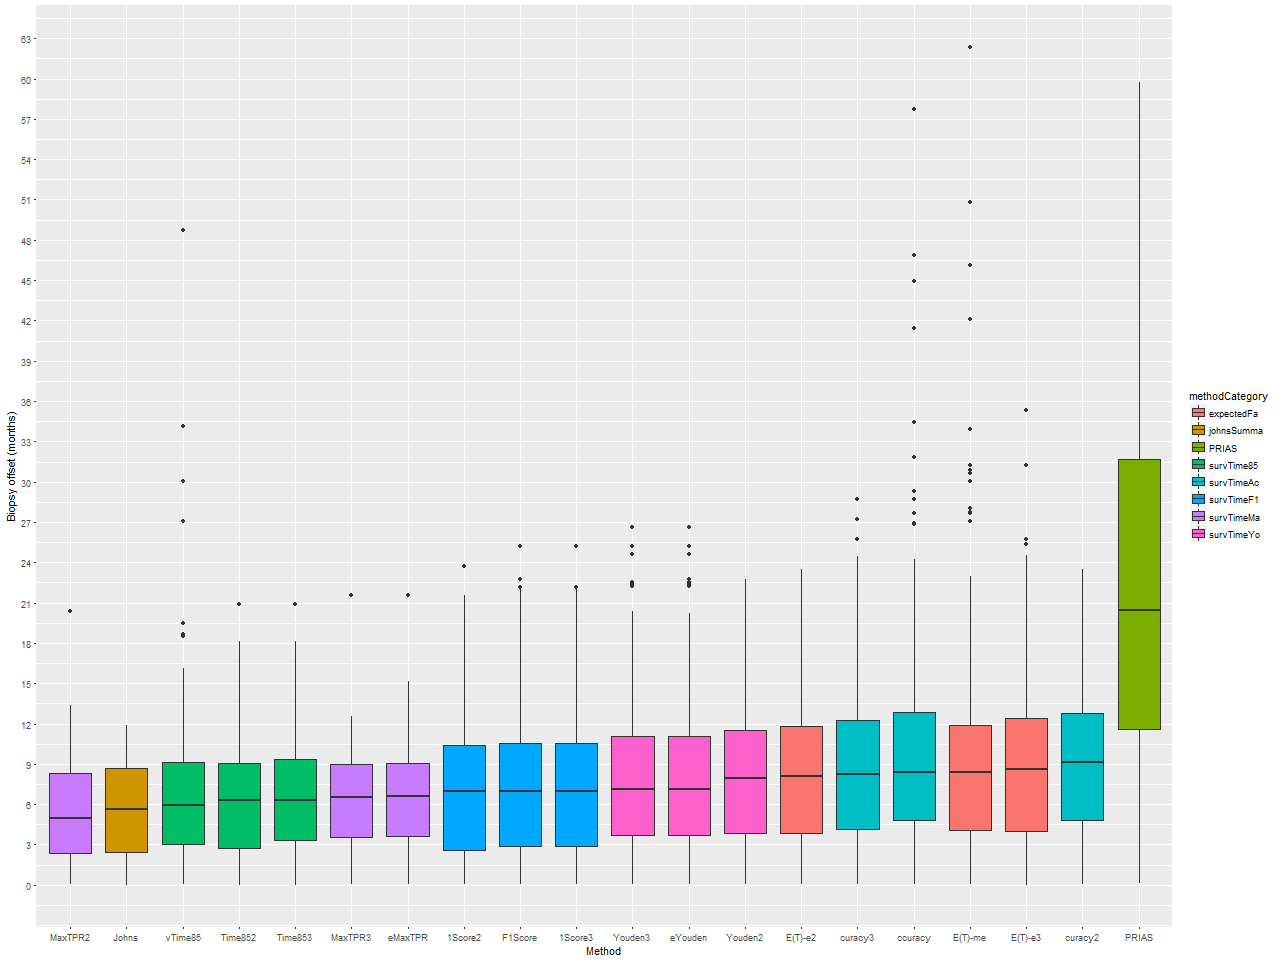
\includegraphics[width=\textwidth]{sim_study_res_sc_10_sh_7pt5/offset_boxplot.png}
\caption{\label{fig : sc_10_sh_7pt5_offset_boxplot} Boxplot for the offset corresponding to the various approaches in scenario 1.}
\end{figure}

\begin{figure}[H]
\centering
\captionsetup{justification=centering}
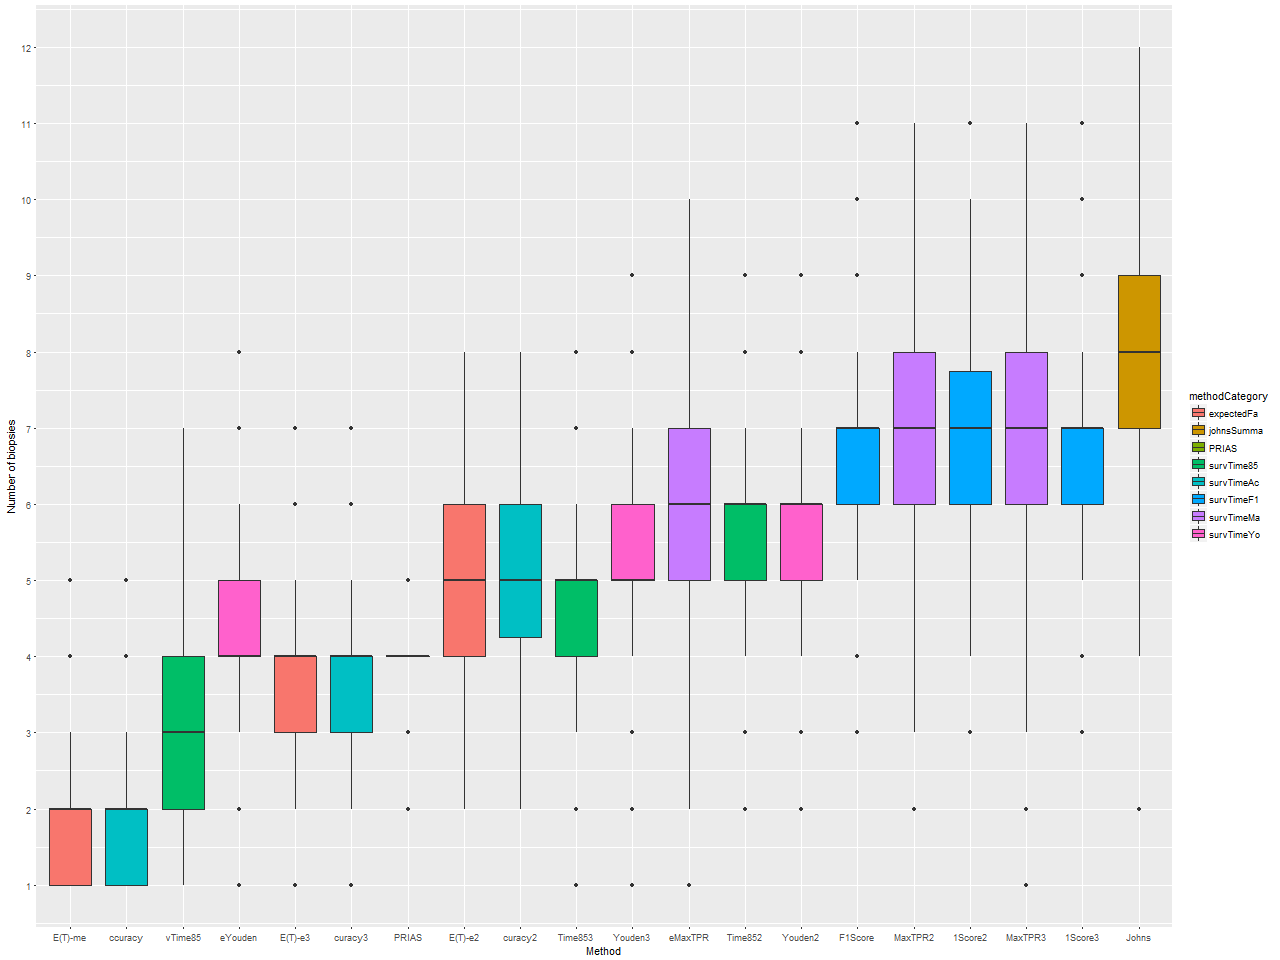
\includegraphics[width=\textwidth]{sim_study_res_sc_10_sh_7pt5/nb_boxplot.png}
\caption{\label{fig : sc_10_sh_7pt5_nb_boxplot} Boxplot for the number of biopsies corresponding to the various approaches in scenario 1.}
\end{figure}

\subsubsection{Scenario 2}
Unlike the previous scenario, the Gleason reclassification times for the patients in Scenario 2 are mostly between 0 and 5 years. The Gleason reclassification times of test patients from one of the data sets is shown in Figure \ref{fig : sc_6_sh_1pt5_progression_hist}. Figure \ref{fig : sc_6_sh_1pt5_offset_boxplot} shows that, for this data set the approach with the least number of biopsies is conditional expected failure time. The mean and median number of biopsies are 1.5 and 1 respectively. While the mean and median offset is around 18 months, there is considerable variation in the offset for the various patients. The first and third quartiles are at 12 months and 27 months respectively. The large variation in offset is due to the fact that time to Gleason reclassification has larger variance since it is based on a small history of the patient. In such a scenario one might be inclined towards doing a biopsy every year as they have the least offset. However that approach leads to a very large number of biopsies as shown in Figure \ref{fig : sc_6_sh_1pt5_nb_boxplot}. Certain approaches based on dynamic risk perform better here, both in terms of number of biopsies as well as the offset. In particular if the choice of $\kappa$ can be based on maximization of the Youden index or a fixed $\kappa$ can be chosen.

\begin{figure}[H]
\centering
\captionsetup{justification=centering}
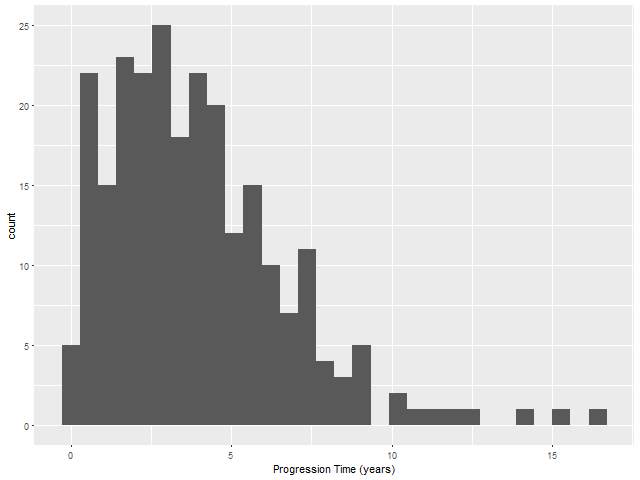
\includegraphics[width=0.8\textwidth]{sim_study_res_sc_6_sh_1pt5/progression_hist.png}
\caption{\label{fig : sc_6_sh_1pt5_progression_hist} Gleason reclassification times for patients from the test data set of scenario 2.}
\end{figure}

\begin{figure}[H]
\centering
\captionsetup{justification=centering}
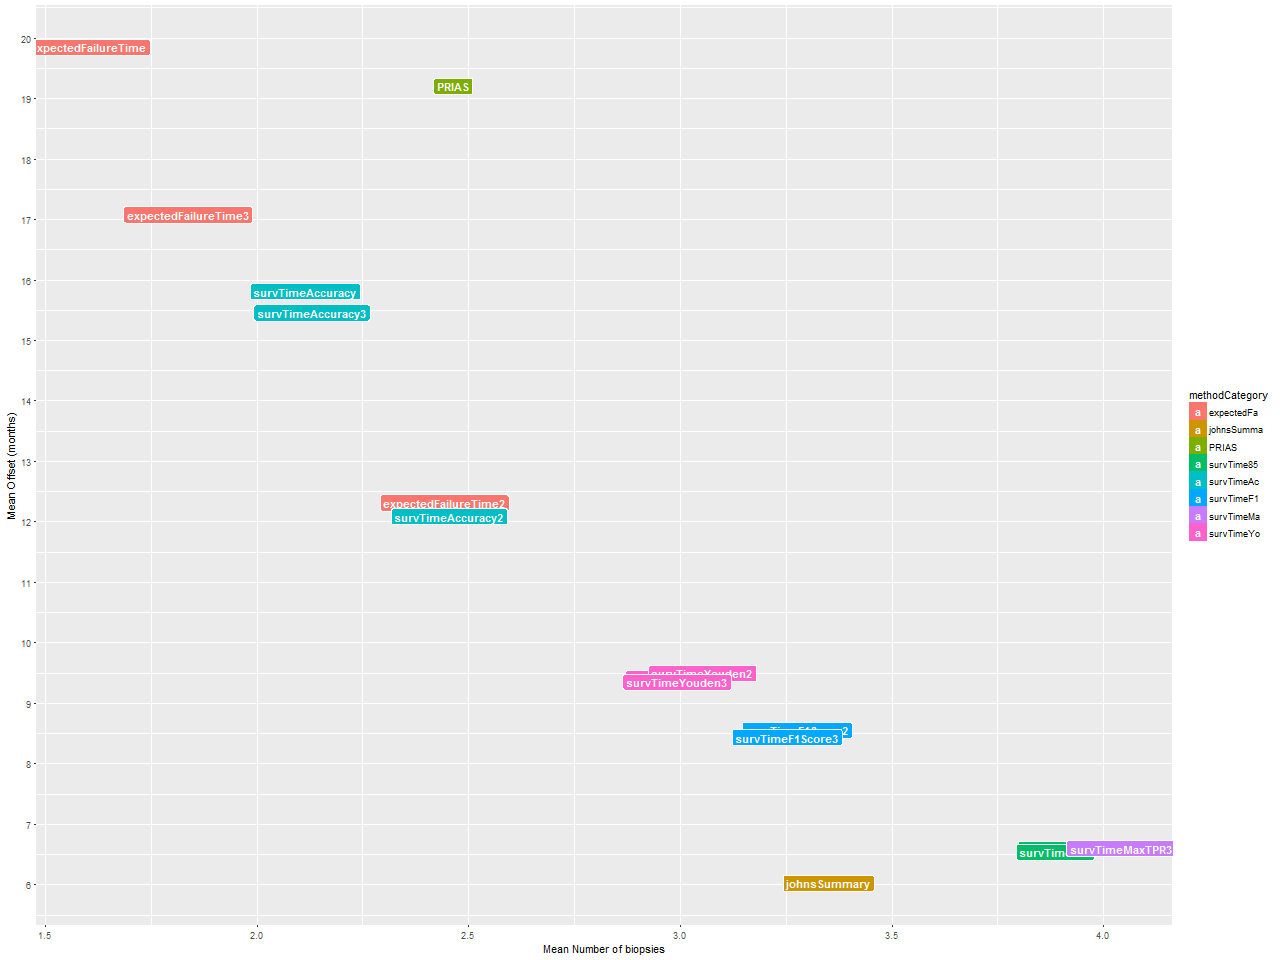
\includegraphics[width=\textwidth]{sim_study_res_sc_6_sh_1pt5/mean_offsetvsnb.png}
\caption{\label{fig : sc_6_sh_1pt5_mean_offsetvsnb} Mean number of biopsies against the mean offset (in years) for each of the approaches in scenario 2.}
\end{figure}

\begin{figure}[H]
\centering
\captionsetup{justification=centering}
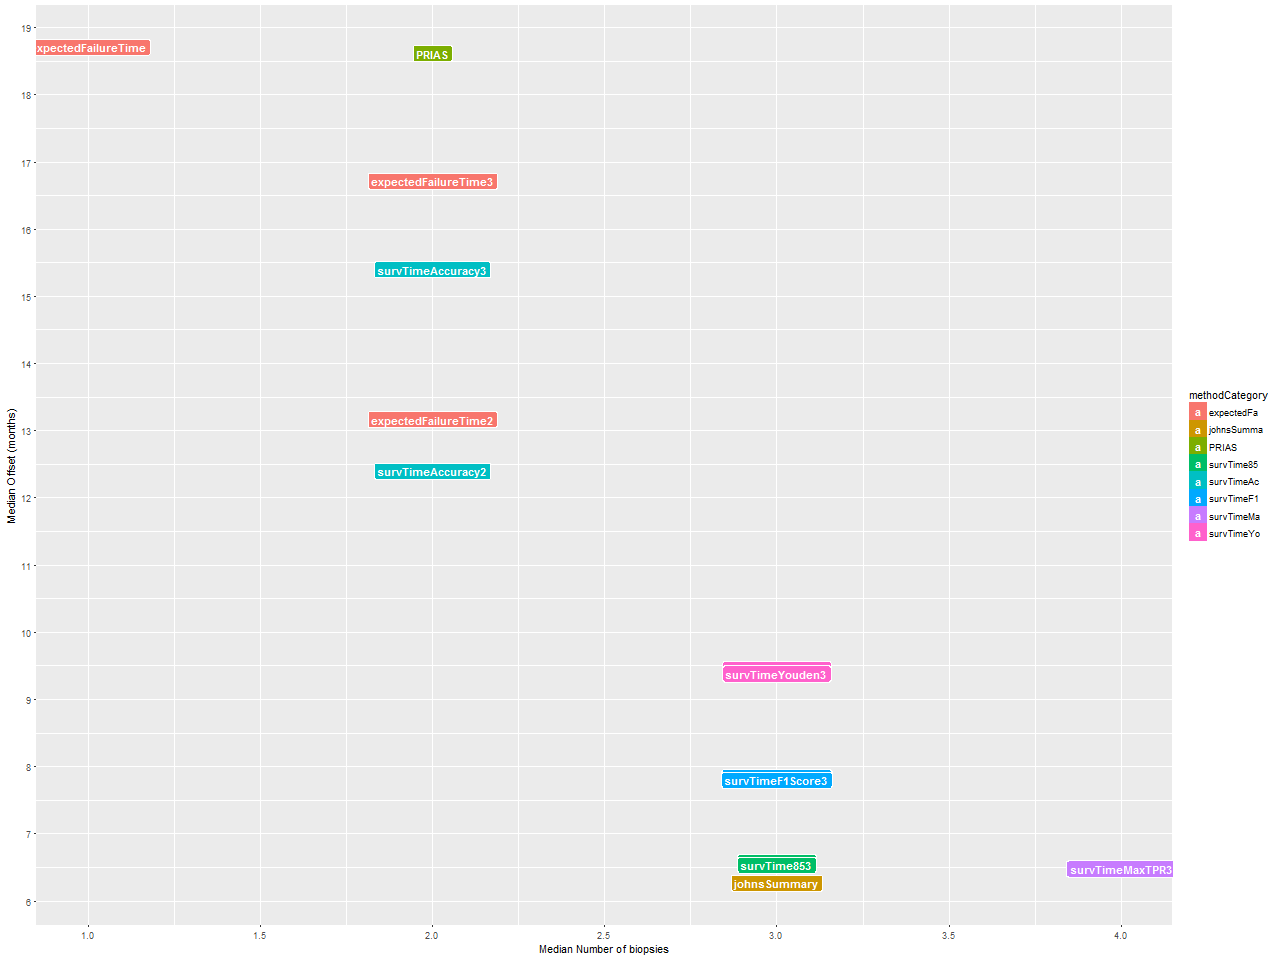
\includegraphics[width=\textwidth]{sim_study_res_sc_6_sh_1pt5/median_offsetvsnb.png}
\caption{\label{fig : sc_6_sh_1pt5_median_offsetvsnb}Median number of biopsies against the median offset (in years) for each of the approaches in scenario 2.}
\end{figure}

\begin{figure}[H]
\centering
\captionsetup{justification=centering}
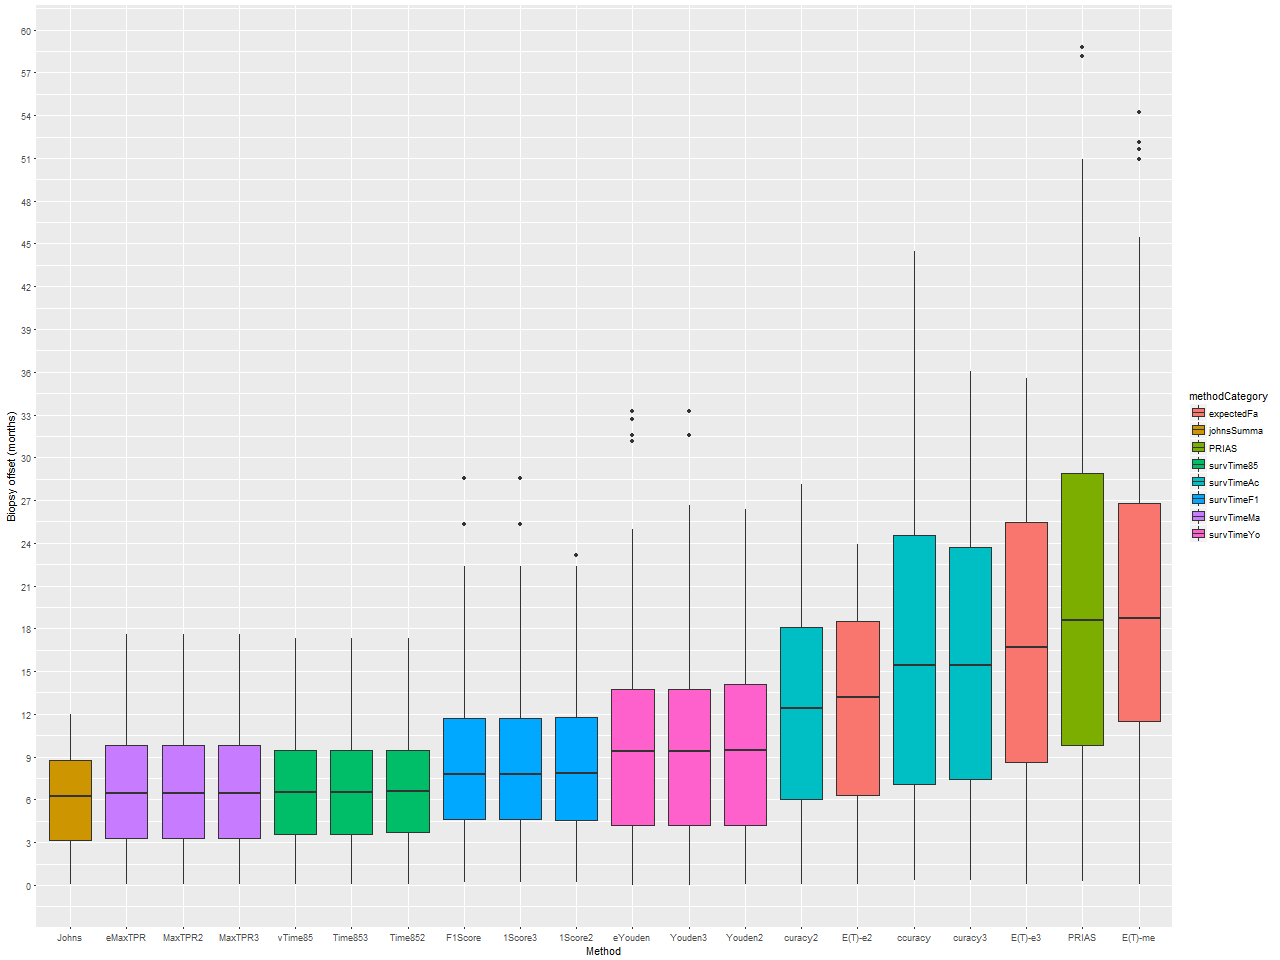
\includegraphics[width=\textwidth]{sim_study_res_sc_6_sh_1pt5/offset_boxplot.png}
\caption{\label{fig : sc_6_sh_1pt5_offset_boxplot} Boxplot for the offset corresponding to the various approaches in scenario 2.}
\end{figure}

\begin{figure}[H]
\centering
\captionsetup{justification=centering}
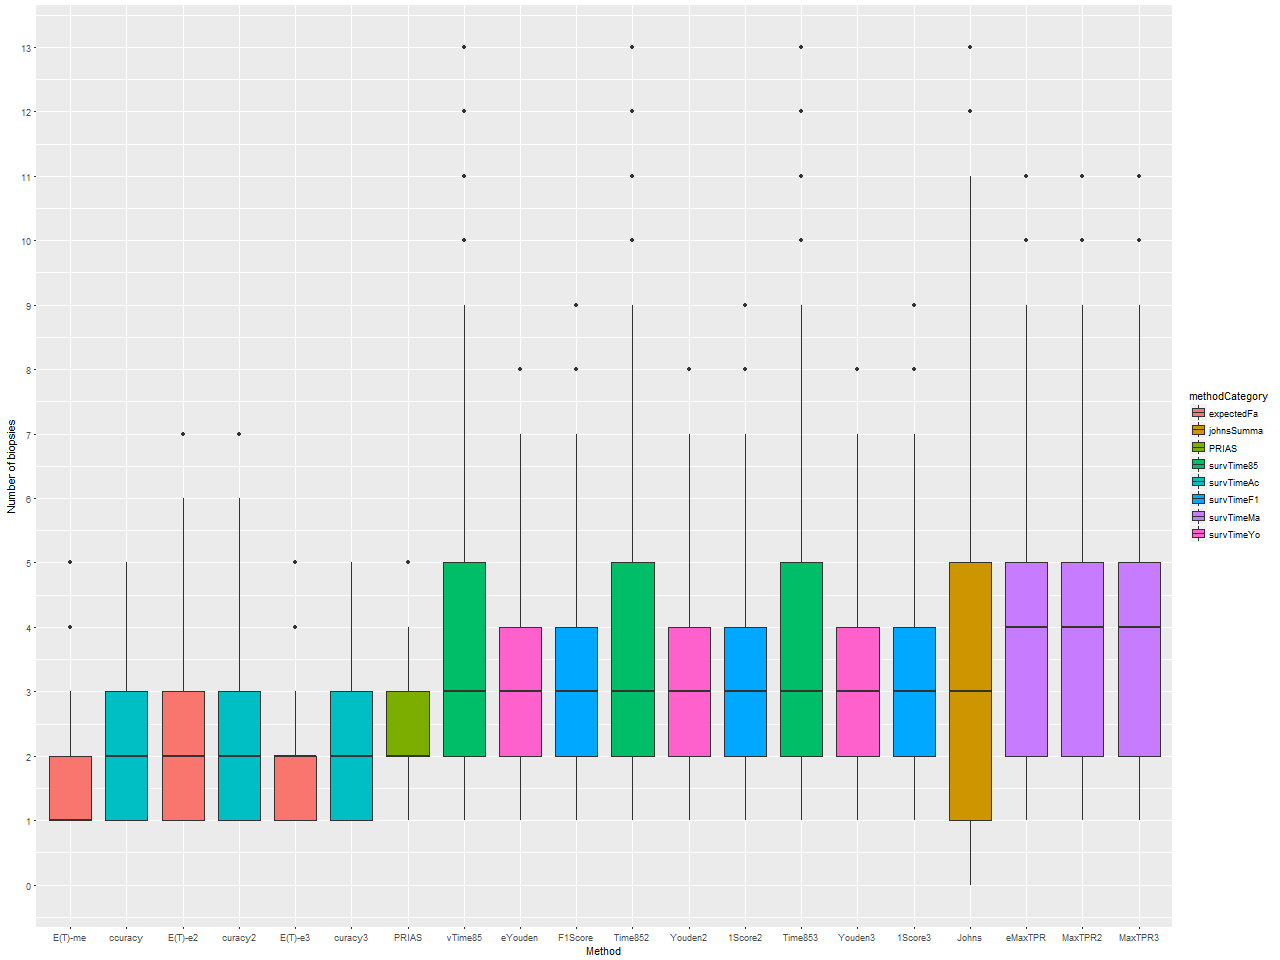
\includegraphics[width=\textwidth]{sim_study_res_sc_6_sh_1pt5/nb_boxplot.png}
\caption{\label{fig : sc_6_sh_1pt5_nb_boxplot} Boxplot for the number of biopsies corresponding to the various approaches in scenario 2.}
\end{figure}

\subsubsection{Scenario 3}
In scenario 3, the Gleason reclassification times for the patients are widely spread, mostly between 2 and 9 years. i.e. patients fail late as well early. The Gleason reclassification times of test patients from one of the data sets is shown in Figure \ref{fig : sc_8pt5_sh_3_progression_hist}. Figure \ref{fig : sc_8pt5_sh_3_offset_boxplot} shows that, for this data set the approach with the least number of biopsies is conditional expected failure time. The mean and median number of biopsies are 1.5 and 1 respectively. This method also has considerable variation in the offset for the various patients. The first and third quartiles are at 9 months and 27 months respectively. A more detailed analysis revealed that the variation in offset was higher for subjects with earlier failure times. For e.g. the mean and median offset in subjects with reclassification times more than 4 years was nearly 13.5 months. For others it was nearly 39.5 months. This is once again is due to the fact that time to Gleason reclassification has larger variance since it is based on a small history of the patient. And thus usefulness of conditional expected failure time is questionable.\\

Dynamic risk based methods once again provide an alternative. If a fixed $\kappa$ of 0.15 is used then although the offset will be low, there is very high variation in number of biopsies. i.e. people who have reclassifications early will benefit but people who have reclassifications later will have too many biopsies. If $\kappa$ is chosen such that accuracy is maximized, and a biopsy is done whenever there is a gap of 2 years then a reasonable offset is obtained. The first and third quartiles are almost 4.5 and 18 months. The first and third quartiles for number of biopsies are 3 and 4. 

\begin{figure}[H]
\centering
\captionsetup{justification=centering}
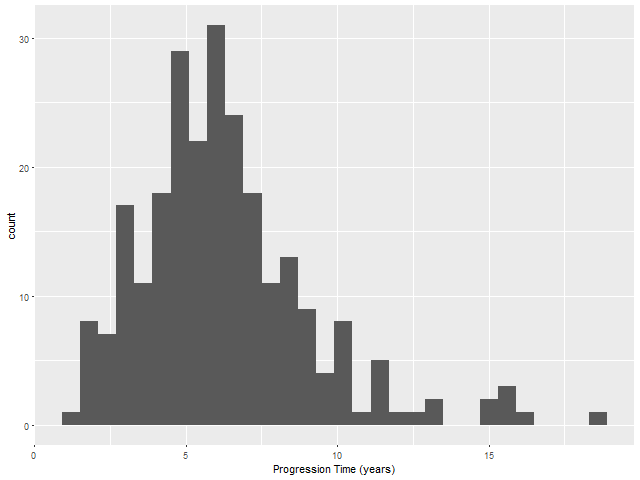
\includegraphics[width=0.8\textwidth]{sim_study_res_sc_8pt5_sh_3/progression_hist.png}
\caption{\label{fig : sc_8pt5_sh_3_progression_hist} Gleason reclassification times for patients from the test data set of scenario 3.}
\end{figure}

\begin{figure}[H]
\centering
\captionsetup{justification=centering}
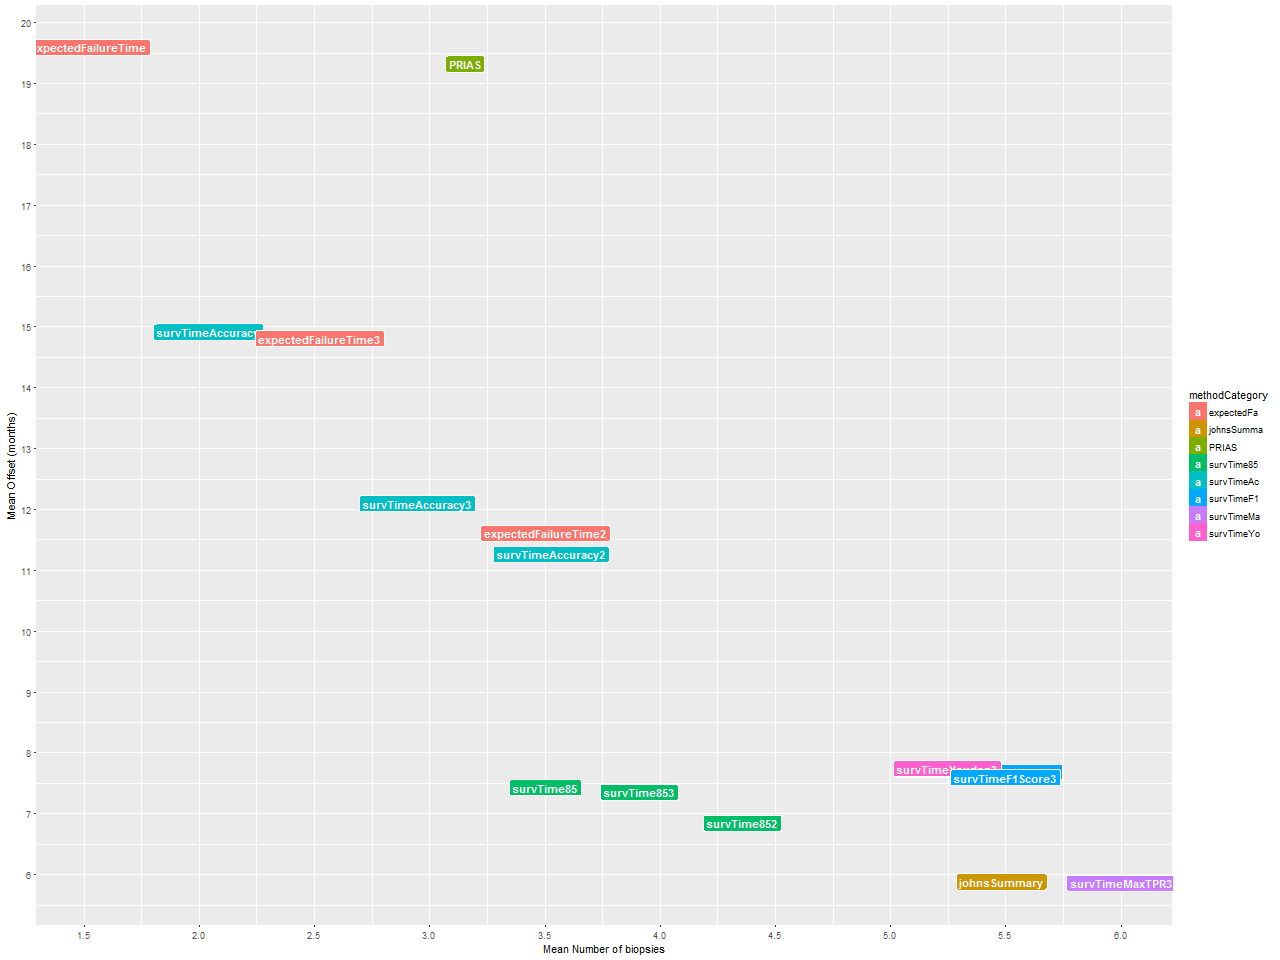
\includegraphics[width=\textwidth]{sim_study_res_sc_8pt5_sh_3/mean_offsetvsnb.png}
\caption{\label{fig : sc_8pt5_sh_3_mean_offsetvsnb} Mean number of biopsies against the mean offset (in years) for each of the approaches in scenario 3.}
\end{figure}

\begin{figure}[H]
\centering
\captionsetup{justification=centering}
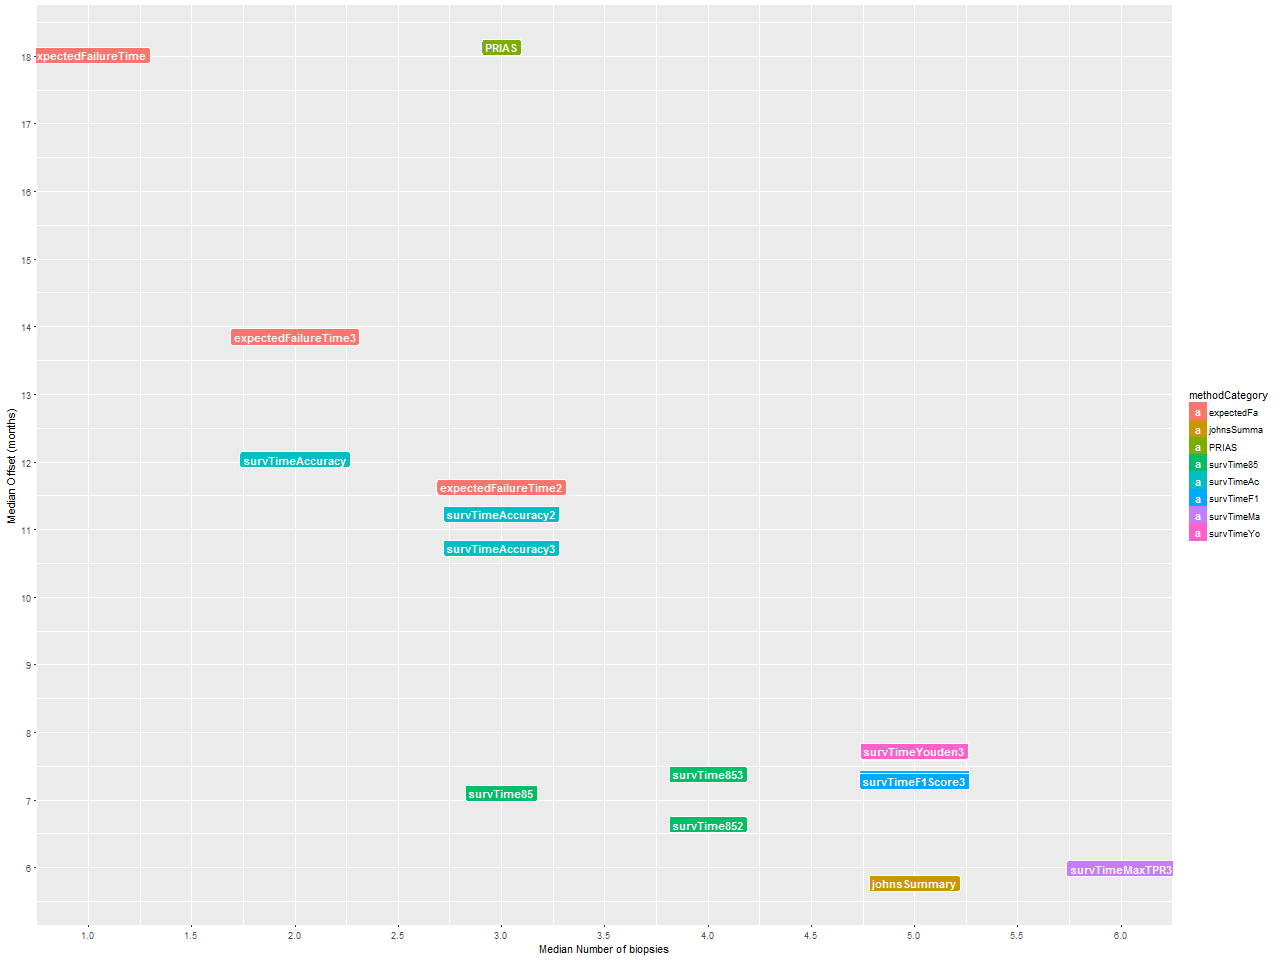
\includegraphics[width=\textwidth]{sim_study_res_sc_8pt5_sh_3/median_offsetvsnb.png}
\caption{\label{fig : sc_8pt5_sh_3_median_offsetvsnb}Median number of biopsies against the median offset (in years) for each of the approaches in scenario 3.}
\end{figure}

\begin{figure}[H]
\centering
\captionsetup{justification=centering}
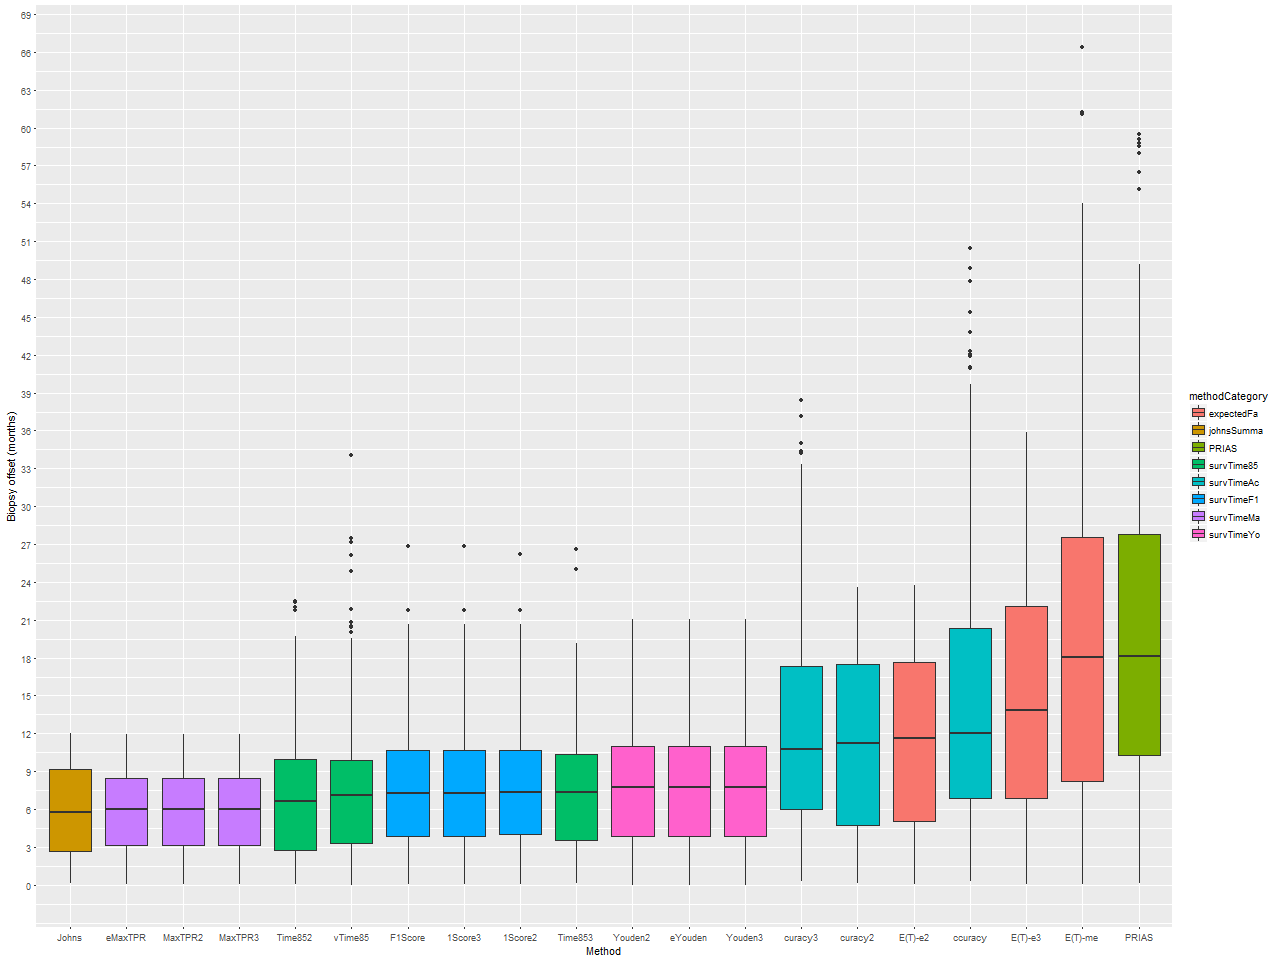
\includegraphics[width=\textwidth]{sim_study_res_sc_8pt5_sh_3/offset_boxplot.png}
\caption{\label{fig : sc_8pt5_sh_3_offset_boxplot} Boxplot for the offset corresponding to the various approaches in scenario 3.}
\end{figure}

\begin{figure}[H]
\centering
\captionsetup{justification=centering}
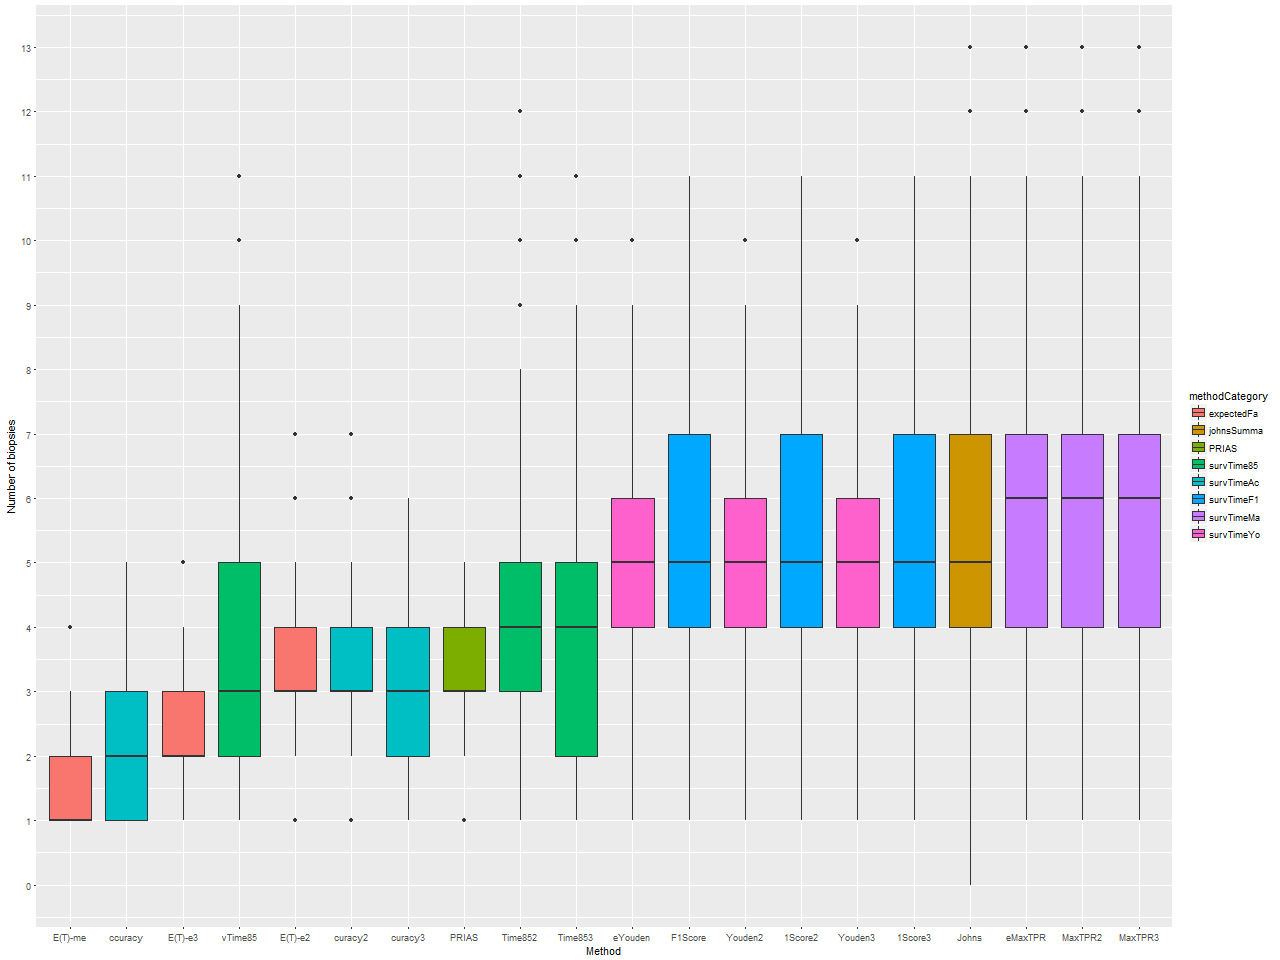
\includegraphics[width=\textwidth]{sim_study_res_sc_8pt5_sh_3/nb_boxplot.png}
\caption{\label{fig : sc_8pt5_sh_3_nb_boxplot} Boxplot for the number of biopsies corresponding to the various approaches in scenario 3.}
\end{figure}